\section{IHM}\label{sec:ihm}

A interface de operação e supervisão foi desenvolvida utilizando o software \textbf{InduSoft Web Studio}, estabelecendo comunicação com o controlador lógico através do driver \textbf{OPC UA} (Porta 4840). O desenvolvimento da tela seguiu os requisitos de animação e controle estipulados nas especificações do projeto.

\subsection{Sinótico Geral e Identidade Visual}
A tela principal apresenta um sinótico completo do processo, integrando as Áreas 01 (Batelada) e 02 (Envase). Para facilitar a interpretação rápida pelo operador, adotou-se a seguinte convenção visual para os atuadores (válvulas e motores):
\begin{itemize}
    \item \textbf{Cor Vermelha:} Indica que o equipamento está \textbf{Ativo/Ligado} ou a válvula está \textbf{Aberta}.
    \item \textbf{Cor Verde:} Indica que o equipamento está \textbf{Desligado} ou a válvula está \textbf{Fechada}.
\end{itemize}

\subsection{Detalhamento das Áreas}

\subsubsection{Reator de Mistura (RM-01)}
O tanque RM-01 possui animações dinâmicas que indicam o nível em tempo real, tanto por preenchimento gráfico vertical (\textit{Bar Graph}) quanto por display numérico em milímetros. O sinótico permite visualizar:
\begin{itemize}
    \item \textbf{Misturador:} O motor do misturador (\textbf{M-101}) altera sua cor quando ligado.
    \item \textbf{Resfriamento:} O estado da jaqueta de resfriamento é monitorado, indicando o estado normal (cinza) ou resfriado (azul claro).
    \item \textbf{Sensores:} O status dos sensores de nível (LSH-101, LSH-102, LSL-101, LSL-102) e temperatura (TSL-101) é indicado por "LEDs" virtuais que alteram de cor conforme a atuação.
\end{itemize}

\subsubsection{Tanque de Produto (TP-01) e Transferência}
O tanque de armazenamento (TP-01) exibe o nível acumulado do produto Dry Martini pronto para o envase. A interface monitora as chaves de nível (LSHH-201, LSH-201, LSL-201) e controla a bomba de transferência \textbf{BA-101}, permitindo ao operador acompanhar o esvaziamento do reator e o enchimento dos barris.

\subsubsection{Sistema de Envase e Transporte (TR-01)}
A esteira transportadora foi animada para representar o fluxo contínuo de produção. Os principais elementos visuais incluem:
\begin{itemize}
    \item \textbf{Movimentação:} Animação dos barris deslocando-se sobre a esteira quando o motor \textbf{M-201} está ativo.
    \item \textbf{Sensores de Proximidade:} Os sensores \textbf{ZY-201} (posicionamento para envase) e \textbf{ZY-202} (contagem de saída) indicam visualmente a detecção dos barris.
    \item \textbf{Bico Injetor:} Animação da válvula \textbf{FV-201} e do fluxo de líquido, que só ocorre quando um barril é validado pelo sensor de posicionamento.
    \item \textbf{Contador de barris:} Indica visualmente a contagem dos barris.
\end{itemize}

\subsection{Modos de Operação e Intertravamentos}

A seleção do modo de operação é realizada através de botões dedicados no painel de comando da IHM, alternando o comportamento do sistema entre \textbf{Automático (AUTO)} e \textbf{Manual (MAN)}:

\begin{itemize}
    \item \textbf{Modo Automático:} Ao ser ativado, o controlador assume a execução lógica da batelada e do envase sequencial. Neste estado, os botões de acionamento individual dos equipamentos (válvulas e motores) são bloqueados na interface, impedindo interferência humana indevida durante a produção.
    
    \item \textbf{Modo Manual:} Ao selecionar este modo, a lógica de sequenciamento é interrompida, e o operador ganha permissão para atuar individualmente sobre cada componente. Na IHM, isso libera o comando de todas as válvulas (FV-101 a FV-107, FV-201), do motor do misturador (M-101), da bomba (BA-101) e do motor do transportador (M-201).
\end{itemize}

Visualmente, a IHM indica o modo ativo, garantindo que o operador esteja sempre ciente do estado de controle da planta.

\subsection{Gerenciamento de Dados e Alarmes}
No canto superior esquerdo, um painel de \textbf{Totalização} exibe os volumes de Gin e Vermouth da batelada atual e os volumes acumulados de Gin, Vermouth e Produto Final ao longo de toda a produção, além de um contador específico para o número de bateladas realizadas.

O sistema conta ainda com:
\begin{itemize}
    \item \textbf{Objeto de Alarmes:} Localizado na parte inferior ("Mensagens"), registra e exibe as falhas e eventos do sistema, ou seja, indica quando o nível do TP-01 está baixo, alto ou muito alto, além de mostrar quando o transportador ficar vazio por mais tempo do que deveria. É possível o operador silenciar ou reconhecer os alarmes dando dois cliques na mensagem.
    \item \textbf{Botão de Emergência:} Disponível em destaque na tela, possui lógica retentiva. Visualmente, o botão indica o estado \textit{True} (acionado/seguro) através da cor \textbf{Verde}, indicando a parada imediata do processo em situações críticas.
\end{itemize}

%  PRINT DA IHM AQUI
\begin{figure}[H]
    \centering
    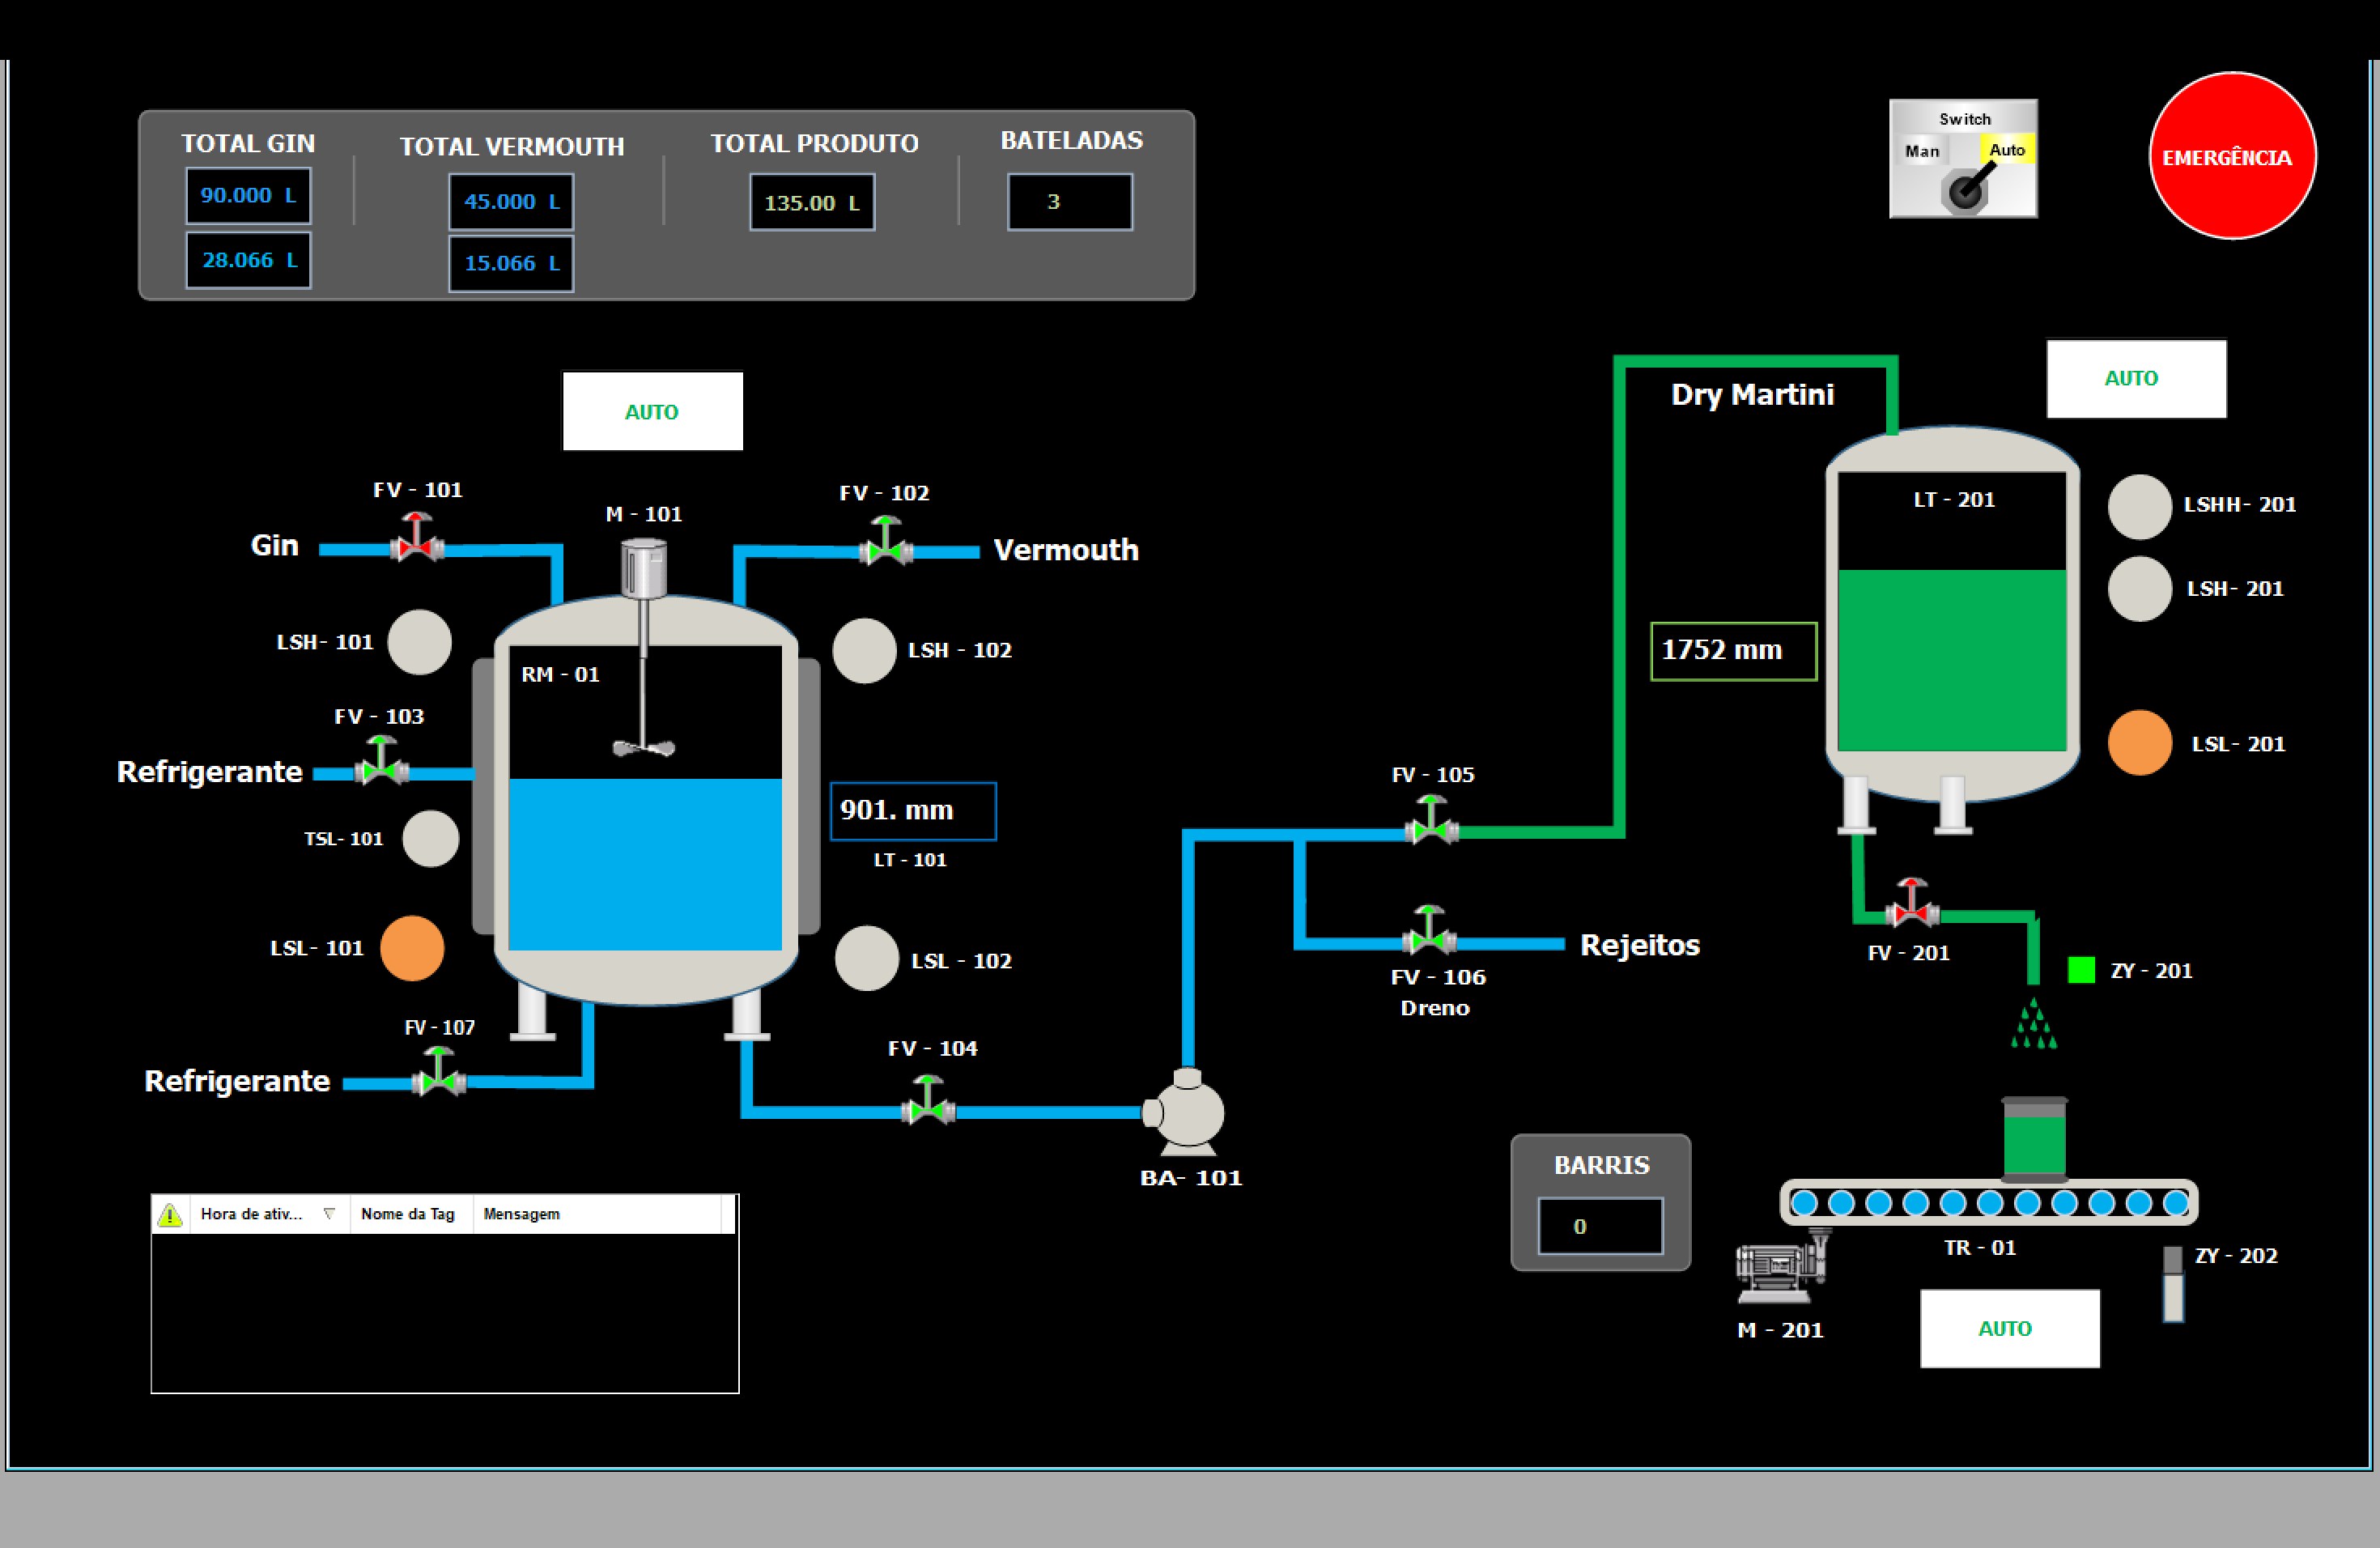
\includegraphics[width=0.8\textwidth]{imgs/print_ihm.png}
    \caption{Tela Principal do Supervisório em funcionamento.}
\end{figure}